\documentclass[twoside]{book}

% Packages required by doxygen
\usepackage{fixltx2e}
\usepackage{calc}
\usepackage{doxygen}
\usepackage[export]{adjustbox} % also loads graphicx
\usepackage{graphicx}
\usepackage[utf8]{inputenc}
\usepackage{makeidx}
\usepackage{multicol}
\usepackage{multirow}
\PassOptionsToPackage{warn}{textcomp}
\usepackage{textcomp}
\usepackage[nointegrals]{wasysym}
\usepackage[table]{xcolor}

% Font selection
\usepackage[T1]{fontenc}
\usepackage[scaled=.90]{helvet}
\usepackage{courier}
\usepackage{amssymb}
\usepackage{sectsty}
\renewcommand{\familydefault}{\sfdefault}
\allsectionsfont{%
  \fontseries{bc}\selectfont%
  \color{darkgray}%
}
\renewcommand{\DoxyLabelFont}{%
  \fontseries{bc}\selectfont%
  \color{darkgray}%
}
\newcommand{\+}{\discretionary{\mbox{\scriptsize$\hookleftarrow$}}{}{}}

% Page & text layout
\usepackage{geometry}
\geometry{%
  a4paper,%
  top=2.5cm,%
  bottom=2.5cm,%
  left=2.5cm,%
  right=2.5cm%
}
\tolerance=750
\hfuzz=15pt
\hbadness=750
\setlength{\emergencystretch}{15pt}
\setlength{\parindent}{0cm}
\setlength{\parskip}{3ex plus 2ex minus 2ex}
\makeatletter
\renewcommand{\paragraph}{%
  \@startsection{paragraph}{4}{0ex}{-1.0ex}{1.0ex}{%
    \normalfont\normalsize\bfseries\SS@parafont%
  }%
}
\renewcommand{\subparagraph}{%
  \@startsection{subparagraph}{5}{0ex}{-1.0ex}{1.0ex}{%
    \normalfont\normalsize\bfseries\SS@subparafont%
  }%
}
\makeatother

% Headers & footers
\usepackage{fancyhdr}
\pagestyle{fancyplain}
\fancyhead[LE]{\fancyplain{}{\bfseries\thepage}}
\fancyhead[CE]{\fancyplain{}{}}
\fancyhead[RE]{\fancyplain{}{\bfseries\leftmark}}
\fancyhead[LO]{\fancyplain{}{\bfseries\rightmark}}
\fancyhead[CO]{\fancyplain{}{}}
\fancyhead[RO]{\fancyplain{}{\bfseries\thepage}}
\fancyfoot[LE]{\fancyplain{}{}}
\fancyfoot[CE]{\fancyplain{}{}}
\fancyfoot[RE]{\fancyplain{}{\bfseries\scriptsize Generated by Doxygen }}
\fancyfoot[LO]{\fancyplain{}{\bfseries\scriptsize Generated by Doxygen }}
\fancyfoot[CO]{\fancyplain{}{}}
\fancyfoot[RO]{\fancyplain{}{}}
\renewcommand{\footrulewidth}{0.4pt}
\renewcommand{\chaptermark}[1]{%
  \markboth{#1}{}%
}
\renewcommand{\sectionmark}[1]{%
  \markright{\thesection\ #1}%
}

% Indices & bibliography
\usepackage{natbib}
\usepackage[titles]{tocloft}
\setcounter{tocdepth}{3}
\setcounter{secnumdepth}{5}
\makeindex

% Hyperlinks (required, but should be loaded last)
\usepackage{ifpdf}
\ifpdf
  \usepackage[pdftex,pagebackref=true]{hyperref}
\else
  \usepackage[ps2pdf,pagebackref=true]{hyperref}
\fi
\hypersetup{%
  colorlinks=true,%
  linkcolor=blue,%
  citecolor=blue,%
  unicode%
}

% Custom commands
\newcommand{\clearemptydoublepage}{%
  \newpage{\pagestyle{empty}\cleardoublepage}%
}

\usepackage{caption}
\captionsetup{labelsep=space,justification=centering,font={bf},singlelinecheck=off,skip=4pt,position=top}

%===== C O N T E N T S =====

\begin{document}

% Titlepage & ToC
\hypersetup{pageanchor=false,
             bookmarksnumbered=true,
             pdfencoding=unicode
            }
\pagenumbering{roman}
\begin{titlepage}
\vspace*{7cm}
\begin{center}%
{\Large Mandelbrot Distributed Program \\[1ex]\large 0.\+0 }\\
\vspace*{1cm}
{\large Generated by Doxygen 1.8.11}\\
\end{center}
\end{titlepage}
\clearemptydoublepage
\tableofcontents
\clearemptydoublepage
\pagenumbering{arabic}
\hypersetup{pageanchor=true}

%--- Begin generated contents ---
\chapter{Bug List}
\label{bug}
\hypertarget{bug}{}

\begin{DoxyRefList}
\item[\label{bug__bug000001}%
\hypertarget{bug__bug000001}{}%
File \hyperlink{mandelbrot__mpi_8c}{mandelbrot\+\_\+mpi.c} ]No known bugs  
\item[\label{bug__bug000002}%
\hypertarget{bug__bug000002}{}%
File \hyperlink{mandelbrot__mpi__io_8c}{mandelbrot\+\_\+mpi\+\_\+io.c} ]No known bugs  
\item[\label{bug__bug000003}%
\hypertarget{bug__bug000003}{}%
File \hyperlink{mandelbrot__mpi__io__pp_8c}{mandelbrot\+\_\+mpi\+\_\+io\+\_\+pp.c} ]No known bugs  
\item[\label{bug__bug000004}%
\hypertarget{bug__bug000004}{}%
File \hyperlink{mandelbrot__mpi__ms_8c}{mandelbrot\+\_\+mpi\+\_\+ms.c} ]No known bugs  
\item[\label{bug__bug000005}%
\hypertarget{bug__bug000005}{}%
File \hyperlink{mandelbrot__mpi__op_8c}{mandelbrot\+\_\+mpi\+\_\+op.c} ]No known bugs  
\item[\label{bug__bug000006}%
\hypertarget{bug__bug000006}{}%
File \hyperlink{mandelbrot__seq_8c}{mandelbrot\+\_\+seq.c} ]No known bugs 
\end{DoxyRefList}
\chapter{File Index}
\section{File List}
Here is a list of all documented files with brief descriptions\+:\begin{DoxyCompactList}
\item\contentsline{section}{\hyperlink{mandelbrot__mpi_8c}{mandelbrot\+\_\+mpi.\+c} \\*Open M\+PI C implementation to compute and plot mandelbrot set }{\pageref{mandelbrot__mpi_8c}}{}
\item\contentsline{section}{\hyperlink{mandelbrot__mpi__io_8c}{mandelbrot\+\_\+mpi\+\_\+io.\+c} \\*Open M\+PI C implementation to compute and plot mandelbrot set }{\pageref{mandelbrot__mpi__io_8c}}{}
\item\contentsline{section}{\hyperlink{mandelbrot__mpi__io__pp_8c}{mandelbrot\+\_\+mpi\+\_\+io\+\_\+pp.\+c} \\*Open M\+PI C implementation to compute and plot mandelbrot set }{\pageref{mandelbrot__mpi__io__pp_8c}}{}
\item\contentsline{section}{\hyperlink{mandelbrot__mpi__ms_8c}{mandelbrot\+\_\+mpi\+\_\+ms.\+c} \\*Open M\+PI C implementation to compute and plot mandelbrot set }{\pageref{mandelbrot__mpi__ms_8c}}{}
\item\contentsline{section}{\hyperlink{mandelbrot__mpi__op_8c}{mandelbrot\+\_\+mpi\+\_\+op.\+c} \\*Open M\+PI C implementation to compute and plot mandelbrot set }{\pageref{mandelbrot__mpi__op_8c}}{}
\item\contentsline{section}{\hyperlink{mandelbrot__seq_8c}{mandelbrot\+\_\+seq.\+c} \\*Sequential program to compute and plot mandelbrot set }{\pageref{mandelbrot__seq_8c}}{}
\end{DoxyCompactList}

\chapter{File Documentation}
\hypertarget{mandelbrot__mpi_8c}{}\section{mandelbrot\+\_\+mpi.\+c File Reference}
\label{mandelbrot__mpi_8c}\index{mandelbrot\+\_\+mpi.\+c@{mandelbrot\+\_\+mpi.\+c}}


Open M\+PI C implementation to compute and plot mandelbrot set.  


{\ttfamily \#include $<$stdio.\+h$>$}\\*
{\ttfamily \#include $<$stdlib.\+h$>$}\\*
{\ttfamily \#include $<$complex.\+h$>$}\\*
{\ttfamily \#include $<$mpi.\+h$>$}\\*
Include dependency graph for mandelbrot\+\_\+mpi.\+c\+:
\nopagebreak
\begin{figure}[H]
\begin{center}
\leavevmode
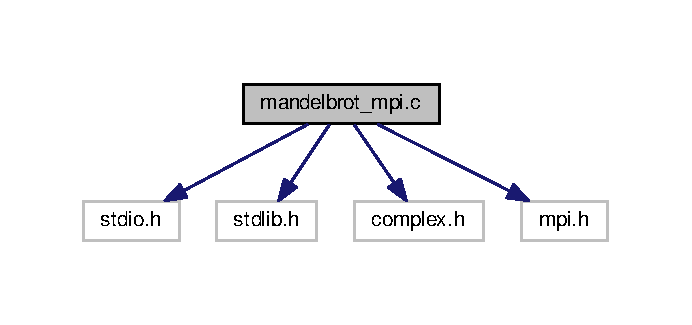
\includegraphics[width=332pt]{mandelbrot__mpi_8c__incl}
\end{center}
\end{figure}
\subsection*{Macros}
\begin{DoxyCompactItemize}
\item 
\#define {\bfseries M\+A\+X\+\_\+\+I\+T\+ER}~300\hypertarget{mandelbrot__mpi_8c_acd517c6f195c75b9dd0f3aad65326f3b}{}\label{mandelbrot__mpi_8c_acd517c6f195c75b9dd0f3aad65326f3b}

\item 
\#define {\bfseries E\+S\+C\+A\+P\+E\+\_\+\+R\+A\+D\+I\+U\+S\+\_\+\+S\+Q\+U\+A\+R\+ED}~4\hypertarget{mandelbrot__mpi_8c_a7c7393421319c3452cfbe9a49a5fbfa7}{}\label{mandelbrot__mpi_8c_a7c7393421319c3452cfbe9a49a5fbfa7}

\end{DoxyCompactItemize}
\subsection*{Functions}
\begin{DoxyCompactItemize}
\item 
int \hyperlink{mandelbrot__mpi_8c_a790aaf32862890d4cd0539c2a77149d6}{mandelbrot} (complex z0)
\begin{DoxyCompactList}\small\item\em Perform the calculations for the set until divergence or M\+A\+X\+\_\+\+I\+T\+ER. \end{DoxyCompactList}\item 
void \hyperlink{mandelbrot__mpi_8c_a2eb771fa3527f72e821a14e413498d1d}{print\+\_\+instructions} ()
\begin{DoxyCompactList}\small\item\em Function responsible for printing usage instructions. \end{DoxyCompactList}\item 
int {\bfseries main} (int argc, char $\ast$$\ast$argv)\hypertarget{mandelbrot__mpi_8c_a3c04138a5bfe5d72780bb7e82a18e627}{}\label{mandelbrot__mpi_8c_a3c04138a5bfe5d72780bb7e82a18e627}

\end{DoxyCompactItemize}


\subsection{Detailed Description}
Open M\+PI C implementation to compute and plot mandelbrot set. 

Open M\+PI C implementation of a program to compute and plot some subset of a mandelbrot set adapted from the classes given by MJ Rutter (\href{https://www.tcm.phy.cam.ac.uk/~mjr/courses/MPI/MPI.pdf}{\tt https\+://www.\+tcm.\+phy.\+cam.\+ac.\+uk/$\sim$mjr/courses/\+M\+P\+I/\+M\+P\+I.\+pdf}) in which every processes is responsible for writing your work

Usage\+: mpirun -\/np NP ./mandelbrot\+\_\+mpi c\+\_\+x\+\_\+min c\+\_\+x\+\_\+max c\+\_\+y\+\_\+min c\+\_\+y\+\_\+max image\+\_\+size
\begin{DoxyItemize}
\item NP\+: Number of Open M\+PI processes
\item c\+\_\+x\+\_\+min\+: Lowest x boundary for the figure to be computed
\item c\+\_\+x\+\_\+max\+: Highest x boundary for the figure to be computed
\item c\+\_\+y\+\_\+mix\+: Lowest y boundary for the figure to be computed
\item c\+\_\+y\+\_\+max\+: Highest y boundary for the figure to be computed
\item image\+\_\+size\+: The resolution of the resulting image Usage examples\+: Full Picture\+: mpirun -\/np 4 ./mandelbrot\+\_\+mpi -\/2.\+5 1.\+5 -\/2.\+0 2.\+0 11500 Seahorse Valley\+: mpirun -\/np 4 ./mandelbrot\+\_\+mpi -\/0.\+8 -\/0.\+7 0.\+05 0.\+15 8192 Elephant Valley\+: mpirun -\/np 8 ./mandelbrot\+\_\+mpi 0.\+175 0.\+375 -\/0.\+1 0.\+1 800 T Spir Val\+: mpirun -\/np 2 ./mandelbrot\+\_\+mpi -\/0.\+188 -\/0.\+012 0.\+554 0.\+754 400
\end{DoxyItemize}

Notes\+: Although we made modifications, this code is heavily based on the class examples provided by MJ Rutter. Because of that, in any event of license and copyright conflict, the license/copyright provided by Mr. Rutter T\+A\+KE P\+R\+E\+C\+E\+D\+E\+N\+CE O\+V\+ER the G\+P\+Lv3 on which this code was released.

\begin{DoxyAuthor}{Author}
Decio Lauro Soares (\href{mailto:deciolauro@gmail.com}{\tt deciolauro@gmail.\+com}) 
\end{DoxyAuthor}
\begin{DoxyDate}{Date}
05 Jul 2017 
\end{DoxyDate}
\begin{DoxyRefDesc}{Bug}
\item[\hyperlink{bug__bug000001}{Bug}]No known bugs \end{DoxyRefDesc}
\begin{DoxyWarning}{Warning}
Based on class given by MJ Rutter(\+May contain Copyright issues) 
\end{DoxyWarning}
\begin{DoxyCopyright}{Copyright}
G\+NU Public License v3 
\end{DoxyCopyright}


\subsection{Function Documentation}
\index{mandelbrot\+\_\+mpi.\+c@{mandelbrot\+\_\+mpi.\+c}!mandelbrot@{mandelbrot}}
\index{mandelbrot@{mandelbrot}!mandelbrot\+\_\+mpi.\+c@{mandelbrot\+\_\+mpi.\+c}}
\subsubsection[{\texorpdfstring{mandelbrot(complex z0)}{mandelbrot(complex z0)}}]{\setlength{\rightskip}{0pt plus 5cm}int mandelbrot (
\begin{DoxyParamCaption}
\item[{complex}]{z0}
\end{DoxyParamCaption}
)}\hypertarget{mandelbrot__mpi_8c_a790aaf32862890d4cd0539c2a77149d6}{}\label{mandelbrot__mpi_8c_a790aaf32862890d4cd0539c2a77149d6}


Perform the calculations for the set until divergence or M\+A\+X\+\_\+\+I\+T\+ER. 

For the complex number z0, it performs the Mandelbrot calculation until it reaches divergence or it reaches the maximum number of iterations, whichever happens first, returning the number of iterations until divergence or M\+A\+X\+\_\+\+I\+T\+ER


\begin{DoxyParams}{Parameters}
{\em z0} & complex number to perform the Mandelbrot calculations \\
\hline
\end{DoxyParams}
\begin{DoxyReturn}{Returns}
i integer with the number of iterations until divergerce or M\+A\+X\+\_\+\+I\+T\+ER 
\end{DoxyReturn}
\index{mandelbrot\+\_\+mpi.\+c@{mandelbrot\+\_\+mpi.\+c}!print\+\_\+instructions@{print\+\_\+instructions}}
\index{print\+\_\+instructions@{print\+\_\+instructions}!mandelbrot\+\_\+mpi.\+c@{mandelbrot\+\_\+mpi.\+c}}
\subsubsection[{\texorpdfstring{print\+\_\+instructions()}{print_instructions()}}]{\setlength{\rightskip}{0pt plus 5cm}void print\+\_\+instructions (
\begin{DoxyParamCaption}
{}
\end{DoxyParamCaption}
)}\hypertarget{mandelbrot__mpi_8c_a2eb771fa3527f72e821a14e413498d1d}{}\label{mandelbrot__mpi_8c_a2eb771fa3527f72e821a14e413498d1d}


Function responsible for printing usage instructions. 

This function is responsible for printing the usage instructions 
\hypertarget{mandelbrot__mpi__io_8c}{}\section{mandelbrot\+\_\+mpi\+\_\+io.\+c File Reference}
\label{mandelbrot__mpi__io_8c}\index{mandelbrot\+\_\+mpi\+\_\+io.\+c@{mandelbrot\+\_\+mpi\+\_\+io.\+c}}


Open M\+PI C implementation to compute and plot mandelbrot set.  


{\ttfamily \#include $<$stdio.\+h$>$}\\*
{\ttfamily \#include $<$stdlib.\+h$>$}\\*
{\ttfamily \#include $<$complex.\+h$>$}\\*
{\ttfamily \#include $<$mpi.\+h$>$}\\*
Include dependency graph for mandelbrot\+\_\+mpi\+\_\+io.\+c\+:
\nopagebreak
\begin{figure}[H]
\begin{center}
\leavevmode
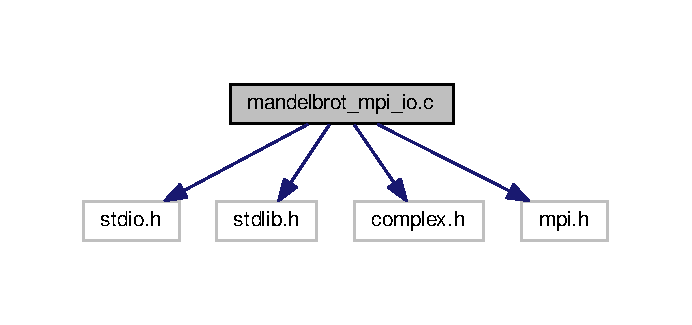
\includegraphics[width=332pt]{mandelbrot__mpi__io_8c__incl}
\end{center}
\end{figure}
\subsection*{Macros}
\begin{DoxyCompactItemize}
\item 
\#define {\bfseries M\+A\+X\+\_\+\+I\+T\+ER}~300\hypertarget{mandelbrot__mpi__io_8c_acd517c6f195c75b9dd0f3aad65326f3b}{}\label{mandelbrot__mpi__io_8c_acd517c6f195c75b9dd0f3aad65326f3b}

\item 
\#define {\bfseries E\+S\+C\+A\+P\+E\+\_\+\+R\+A\+D\+I\+U\+S\+\_\+\+S\+Q\+U\+A\+R\+ED}~4\hypertarget{mandelbrot__mpi__io_8c_a7c7393421319c3452cfbe9a49a5fbfa7}{}\label{mandelbrot__mpi__io_8c_a7c7393421319c3452cfbe9a49a5fbfa7}

\end{DoxyCompactItemize}
\subsection*{Functions}
\begin{DoxyCompactItemize}
\item 
int \hyperlink{mandelbrot__mpi__io_8c_a790aaf32862890d4cd0539c2a77149d6}{mandelbrot} (complex z0)
\begin{DoxyCompactList}\small\item\em Perform the calculations for the set until divergence or M\+A\+X\+\_\+\+I\+T\+ER. \end{DoxyCompactList}\item 
void \hyperlink{mandelbrot__mpi__io_8c_a2eb771fa3527f72e821a14e413498d1d}{print\+\_\+instructions} ()
\begin{DoxyCompactList}\small\item\em Function responsible for printing usage instructions. \end{DoxyCompactList}\item 
int {\bfseries main} (int argc, char $\ast$$\ast$argv)\hypertarget{mandelbrot__mpi__io_8c_a3c04138a5bfe5d72780bb7e82a18e627}{}\label{mandelbrot__mpi__io_8c_a3c04138a5bfe5d72780bb7e82a18e627}

\end{DoxyCompactItemize}


\subsection{Detailed Description}
Open M\+PI C implementation to compute and plot mandelbrot set. 

Open M\+PI C implementation of a program to compute and plot some subset of a mandelbrot set adapted from the classes given by MJ Rutter (\href{https://www.tcm.phy.cam.ac.uk/~mjr/courses/MPI/MPI.pdf}{\tt https\+://www.\+tcm.\+phy.\+cam.\+ac.\+uk/$\sim$mjr/courses/\+M\+P\+I/\+M\+P\+I.\+pdf}) in which process zero is the only responsible for the I/O operations by using the M\+P\+I\+\_\+\+Gather call and a buffer to keep the transfer

Usage\+: mpirun -\/np NP ./mandelbrot\+\_\+mpi\+\_\+io c\+\_\+x\+\_\+min c\+\_\+x\+\_\+max c\+\_\+y\+\_\+min c\+\_\+y\+\_\+max image\+\_\+size
\begin{DoxyItemize}
\item NP\+: Number of Open M\+PI processes
\item c\+\_\+x\+\_\+min\+: Lowest x boundary for the figure to be computed
\item c\+\_\+x\+\_\+max\+: Highest x boundary for the figure to be computed
\item c\+\_\+y\+\_\+mix\+: Lowest y boundary for the figure to be computed
\item c\+\_\+y\+\_\+max\+: Highest y boundary for the figure to be computed
\item image\+\_\+size\+: The resolution of the resulting image Usage examples\+: Full Picture\+: mpirun -\/np 4 ./mandelbrot\+\_\+mpi\+\_\+io -\/2.\+5 1.\+5 -\/2.\+0 2.\+0 11500 Seahorse Valley\+: mpirun -\/np 4 ./mandelbrot\+\_\+mpi\+\_\+io -\/0.\+8 -\/0.\+7 0.\+05 0.\+15 8192 Elephant Valley\+: mpirun -\/np 8 ./mandelbrot\+\_\+mpi\+\_\+io 0.\+175 0.\+375 -\/0.\+1 0.\+1 800 TS Valley\+: mpirun -\/np 2 ./mandelbrot\+\_\+mpi\+\_\+io -\/0.\+188 -\/0.\+012 0.\+554 0.\+754 400
\end{DoxyItemize}

Notes\+: Although we made modifications, this code is heavily based on the class examples provided by MJ Rutter. Because of that, in any event of license and copyright conflict, the license/copyright provided by Mr. Rutter T\+A\+KE P\+R\+E\+C\+E\+D\+E\+N\+CE O\+V\+ER the G\+P\+Lv3 on which this code was released.

\begin{DoxyAuthor}{Author}
Decio Lauro Soares (\href{mailto:deciolauro@gmail.com}{\tt deciolauro@gmail.\+com}) 
\end{DoxyAuthor}
\begin{DoxyDate}{Date}
05 Jul 2017 
\end{DoxyDate}
\begin{DoxyRefDesc}{Bug}
\item[\hyperlink{bug__bug000002}{Bug}]No known bugs \end{DoxyRefDesc}
\begin{DoxyWarning}{Warning}
Based on class given by MJ Rutter(\+May contain Copyright issues) 
\end{DoxyWarning}
\begin{DoxyCopyright}{Copyright}
G\+NU Public License v3 
\end{DoxyCopyright}


\subsection{Function Documentation}
\index{mandelbrot\+\_\+mpi\+\_\+io.\+c@{mandelbrot\+\_\+mpi\+\_\+io.\+c}!mandelbrot@{mandelbrot}}
\index{mandelbrot@{mandelbrot}!mandelbrot\+\_\+mpi\+\_\+io.\+c@{mandelbrot\+\_\+mpi\+\_\+io.\+c}}
\subsubsection[{\texorpdfstring{mandelbrot(complex z0)}{mandelbrot(complex z0)}}]{\setlength{\rightskip}{0pt plus 5cm}int mandelbrot (
\begin{DoxyParamCaption}
\item[{complex}]{z0}
\end{DoxyParamCaption}
)}\hypertarget{mandelbrot__mpi__io_8c_a790aaf32862890d4cd0539c2a77149d6}{}\label{mandelbrot__mpi__io_8c_a790aaf32862890d4cd0539c2a77149d6}


Perform the calculations for the set until divergence or M\+A\+X\+\_\+\+I\+T\+ER. 

For the complex number z0, it performs the Mandelbrot calculation until it reaches divergence or it reaches the maximum number of iterations, whichever happens first, returning the number of iterations until divergence or M\+A\+X\+\_\+\+I\+T\+ER


\begin{DoxyParams}{Parameters}
{\em z0} & complex number to perform the Mandelbrot calculations \\
\hline
\end{DoxyParams}
\begin{DoxyReturn}{Returns}
i integer with the number of iterations until divergerce or M\+A\+X\+\_\+\+I\+T\+ER 
\end{DoxyReturn}
\index{mandelbrot\+\_\+mpi\+\_\+io.\+c@{mandelbrot\+\_\+mpi\+\_\+io.\+c}!print\+\_\+instructions@{print\+\_\+instructions}}
\index{print\+\_\+instructions@{print\+\_\+instructions}!mandelbrot\+\_\+mpi\+\_\+io.\+c@{mandelbrot\+\_\+mpi\+\_\+io.\+c}}
\subsubsection[{\texorpdfstring{print\+\_\+instructions()}{print_instructions()}}]{\setlength{\rightskip}{0pt plus 5cm}void print\+\_\+instructions (
\begin{DoxyParamCaption}
{}
\end{DoxyParamCaption}
)}\hypertarget{mandelbrot__mpi__io_8c_a2eb771fa3527f72e821a14e413498d1d}{}\label{mandelbrot__mpi__io_8c_a2eb771fa3527f72e821a14e413498d1d}


Function responsible for printing usage instructions. 

This function is responsible for printing the usage instructions 
\hypertarget{mandelbrot__mpi__io__pp_8c}{}\section{mandelbrot\+\_\+mpi\+\_\+io\+\_\+pp.\+c File Reference}
\label{mandelbrot__mpi__io__pp_8c}\index{mandelbrot\+\_\+mpi\+\_\+io\+\_\+pp.\+c@{mandelbrot\+\_\+mpi\+\_\+io\+\_\+pp.\+c}}


Open M\+PI C implementation to compute and plot mandelbrot set.  


{\ttfamily \#include $<$stdio.\+h$>$}\\*
{\ttfamily \#include $<$stdlib.\+h$>$}\\*
{\ttfamily \#include $<$complex.\+h$>$}\\*
{\ttfamily \#include $<$mpi.\+h$>$}\\*
Include dependency graph for mandelbrot\+\_\+mpi\+\_\+io\+\_\+pp.\+c\+:
\nopagebreak
\begin{figure}[H]
\begin{center}
\leavevmode
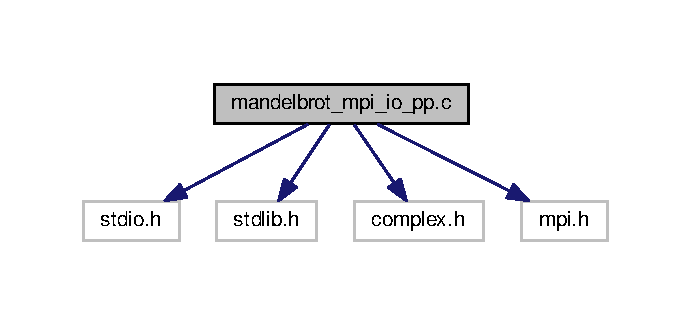
\includegraphics[width=332pt]{mandelbrot__mpi__io__pp_8c__incl}
\end{center}
\end{figure}
\subsection*{Macros}
\begin{DoxyCompactItemize}
\item 
\#define {\bfseries M\+A\+X\+\_\+\+I\+T\+ER}~300\hypertarget{mandelbrot__mpi__io__pp_8c_acd517c6f195c75b9dd0f3aad65326f3b}{}\label{mandelbrot__mpi__io__pp_8c_acd517c6f195c75b9dd0f3aad65326f3b}

\item 
\#define {\bfseries E\+S\+C\+A\+P\+E\+\_\+\+R\+A\+D\+I\+U\+S\+\_\+\+S\+Q\+U\+A\+R\+ED}~4\hypertarget{mandelbrot__mpi__io__pp_8c_a7c7393421319c3452cfbe9a49a5fbfa7}{}\label{mandelbrot__mpi__io__pp_8c_a7c7393421319c3452cfbe9a49a5fbfa7}

\end{DoxyCompactItemize}
\subsection*{Functions}
\begin{DoxyCompactItemize}
\item 
int \hyperlink{mandelbrot__mpi__io__pp_8c_a790aaf32862890d4cd0539c2a77149d6}{mandelbrot} (complex z0)
\begin{DoxyCompactList}\small\item\em Perform the calculations for the set until divergence or M\+A\+X\+\_\+\+I\+T\+ER. \end{DoxyCompactList}\item 
void \hyperlink{mandelbrot__mpi__io__pp_8c_a2eb771fa3527f72e821a14e413498d1d}{print\+\_\+instructions} ()
\begin{DoxyCompactList}\small\item\em Function responsible for printing usage instructions. \end{DoxyCompactList}\item 
int {\bfseries main} (int argc, char $\ast$$\ast$argv)\hypertarget{mandelbrot__mpi__io__pp_8c_a3c04138a5bfe5d72780bb7e82a18e627}{}\label{mandelbrot__mpi__io__pp_8c_a3c04138a5bfe5d72780bb7e82a18e627}

\end{DoxyCompactItemize}


\subsection{Detailed Description}
Open M\+PI C implementation to compute and plot mandelbrot set. 

Open M\+PI C implementation of a program to compute and plot some subset of a mandelbrot set adapted from the classes given by MJ Rutter (\href{https://www.tcm.phy.cam.ac.uk/~mjr/courses/MPI/MPI.pdf}{\tt https\+://www.\+tcm.\+phy.\+cam.\+ac.\+uk/$\sim$mjr/courses/\+M\+P\+I/\+M\+P\+I.\+pdf}) in which process zero is the only responsible for the I/O operations by using point-\/to-\/point M\+PI calls and no memory buffer

Usage\+: mpirun -\/np NP ./mandelbrot\+\_\+mpi\+\_\+io\+\_\+pp c\+\_\+x\+\_\+min c\+\_\+x\+\_\+max c\+\_\+y\+\_\+min c\+\_\+y\+\_\+max image\+\_\+size
\begin{DoxyItemize}
\item NP\+: Number of Open M\+PI processes
\item c\+\_\+x\+\_\+min\+: Lowest x boundary for the figure to be computed
\item c\+\_\+x\+\_\+max\+: Highest x boundary for the figure to be computed
\item c\+\_\+y\+\_\+mix\+: Lowest y boundary for the figure to be computed
\item c\+\_\+y\+\_\+max\+: Highest y boundary for the figure to be computed
\item image\+\_\+size\+: The resolution of the resulting image Usage examples\+: Full Picture\+: mpirun -\/np 4 ./mandelbrot\+\_\+mpi\+\_\+io\+\_\+pp -\/2.\+5 1.\+5 -\/2.\+0 2.\+0 11500 Seahorse Valley\+: mpirun -\/np 4 ./mandelbrot\+\_\+mpi\+\_\+io\+\_\+pp -\/0.\+8 -\/0.\+7 0.\+05 0.\+15 8192 Elephant Valley\+: mpirun -\/np 8 ./mandelbrot\+\_\+mpi\+\_\+io\+\_\+pp 0.\+175 0.\+375 -\/0.\+1 0.\+1 800 TS Valley\+: mpirun -\/np 2 ./mandelbrot\+\_\+mpi\+\_\+io\+\_\+pp -\/0.\+188 -\/0.\+012 0.\+554 0.\+754 400
\end{DoxyItemize}

Notes\+: Although we made modifications, this code is heavily based on the class examples provided by MJ Rutter. Because of that, in any event of license and copyright conflict, the license/copyright provided by Mr. Rutter T\+A\+KE P\+R\+E\+C\+E\+D\+E\+N\+CE O\+V\+ER the G\+P\+Lv3 on which this code was released.

\begin{DoxyAuthor}{Author}
Decio Lauro Soares (\href{mailto:deciolauro@gmail.com}{\tt deciolauro@gmail.\+com}) 
\end{DoxyAuthor}
\begin{DoxyDate}{Date}
05 Jul 2017 
\end{DoxyDate}
\begin{DoxyRefDesc}{Bug}
\item[\hyperlink{bug__bug000003}{Bug}]No known bugs \end{DoxyRefDesc}
\begin{DoxyWarning}{Warning}
Based on class given by MJ Rutter(\+May contain Copyright issues) 
\end{DoxyWarning}
\begin{DoxyCopyright}{Copyright}
G\+NU Public License v3 
\end{DoxyCopyright}


\subsection{Function Documentation}
\index{mandelbrot\+\_\+mpi\+\_\+io\+\_\+pp.\+c@{mandelbrot\+\_\+mpi\+\_\+io\+\_\+pp.\+c}!mandelbrot@{mandelbrot}}
\index{mandelbrot@{mandelbrot}!mandelbrot\+\_\+mpi\+\_\+io\+\_\+pp.\+c@{mandelbrot\+\_\+mpi\+\_\+io\+\_\+pp.\+c}}
\subsubsection[{\texorpdfstring{mandelbrot(complex z0)}{mandelbrot(complex z0)}}]{\setlength{\rightskip}{0pt plus 5cm}int mandelbrot (
\begin{DoxyParamCaption}
\item[{complex}]{z0}
\end{DoxyParamCaption}
)}\hypertarget{mandelbrot__mpi__io__pp_8c_a790aaf32862890d4cd0539c2a77149d6}{}\label{mandelbrot__mpi__io__pp_8c_a790aaf32862890d4cd0539c2a77149d6}


Perform the calculations for the set until divergence or M\+A\+X\+\_\+\+I\+T\+ER. 

For the complex number z0, it performs the Mandelbrot calculation until it reaches divergence or it reaches the maximum number of iterations, whichever happens first, returning the number of iterations until divergence or M\+A\+X\+\_\+\+I\+T\+ER


\begin{DoxyParams}{Parameters}
{\em z0} & complex number to perform the Mandelbrot calculations \\
\hline
\end{DoxyParams}
\begin{DoxyReturn}{Returns}
i integer with the number of iterations until divergerce or M\+A\+X\+\_\+\+I\+T\+ER 
\end{DoxyReturn}
\index{mandelbrot\+\_\+mpi\+\_\+io\+\_\+pp.\+c@{mandelbrot\+\_\+mpi\+\_\+io\+\_\+pp.\+c}!print\+\_\+instructions@{print\+\_\+instructions}}
\index{print\+\_\+instructions@{print\+\_\+instructions}!mandelbrot\+\_\+mpi\+\_\+io\+\_\+pp.\+c@{mandelbrot\+\_\+mpi\+\_\+io\+\_\+pp.\+c}}
\subsubsection[{\texorpdfstring{print\+\_\+instructions()}{print_instructions()}}]{\setlength{\rightskip}{0pt plus 5cm}void print\+\_\+instructions (
\begin{DoxyParamCaption}
{}
\end{DoxyParamCaption}
)}\hypertarget{mandelbrot__mpi__io__pp_8c_a2eb771fa3527f72e821a14e413498d1d}{}\label{mandelbrot__mpi__io__pp_8c_a2eb771fa3527f72e821a14e413498d1d}


Function responsible for printing usage instructions. 

This function is responsible for printing the usage instructions 
\hypertarget{mandelbrot__mpi__ms_8c}{}\section{mandelbrot\+\_\+mpi\+\_\+ms.\+c File Reference}
\label{mandelbrot__mpi__ms_8c}\index{mandelbrot\+\_\+mpi\+\_\+ms.\+c@{mandelbrot\+\_\+mpi\+\_\+ms.\+c}}


Open M\+PI C implementation to compute and plot mandelbrot set.  


{\ttfamily \#include $<$stdio.\+h$>$}\\*
{\ttfamily \#include $<$stdlib.\+h$>$}\\*
{\ttfamily \#include $<$complex.\+h$>$}\\*
{\ttfamily \#include $<$mpi.\+h$>$}\\*
Include dependency graph for mandelbrot\+\_\+mpi\+\_\+ms.\+c\+:
\nopagebreak
\begin{figure}[H]
\begin{center}
\leavevmode
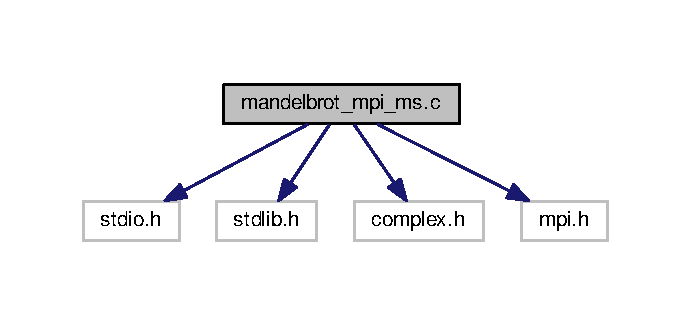
\includegraphics[width=332pt]{mandelbrot__mpi__ms_8c__incl}
\end{center}
\end{figure}
\subsection*{Macros}
\begin{DoxyCompactItemize}
\item 
\#define {\bfseries M\+A\+X\+\_\+\+I\+T\+ER}~300\hypertarget{mandelbrot__mpi__ms_8c_acd517c6f195c75b9dd0f3aad65326f3b}{}\label{mandelbrot__mpi__ms_8c_acd517c6f195c75b9dd0f3aad65326f3b}

\item 
\#define {\bfseries E\+S\+C\+A\+P\+E\+\_\+\+R\+A\+D\+I\+U\+S\+\_\+\+S\+Q\+U\+A\+R\+ED}~4\hypertarget{mandelbrot__mpi__ms_8c_a7c7393421319c3452cfbe9a49a5fbfa7}{}\label{mandelbrot__mpi__ms_8c_a7c7393421319c3452cfbe9a49a5fbfa7}

\end{DoxyCompactItemize}
\subsection*{Functions}
\begin{DoxyCompactItemize}
\item 
int \hyperlink{mandelbrot__mpi__ms_8c_a790aaf32862890d4cd0539c2a77149d6}{mandelbrot} (complex z0)
\begin{DoxyCompactList}\small\item\em Perform the calculations for the set until divergence or M\+A\+X\+\_\+\+I\+T\+ER. \end{DoxyCompactList}\item 
void \hyperlink{mandelbrot__mpi__ms_8c_a2eb771fa3527f72e821a14e413498d1d}{print\+\_\+instructions} ()
\begin{DoxyCompactList}\small\item\em Function responsible for printing usage instructions. \end{DoxyCompactList}\item 
int {\bfseries main} (int argc, char $\ast$$\ast$argv)\hypertarget{mandelbrot__mpi__ms_8c_a3c04138a5bfe5d72780bb7e82a18e627}{}\label{mandelbrot__mpi__ms_8c_a3c04138a5bfe5d72780bb7e82a18e627}

\end{DoxyCompactItemize}


\subsection{Detailed Description}
Open M\+PI C implementation to compute and plot mandelbrot set. 

Open M\+PI C implementation of a program to compute and plot some subset of a mandelbrot set adapted from the classes given by MJ Rutter (\href{https://www.tcm.phy.cam.ac.uk/~mjr/courses/MPI/MPI.pdf}{\tt https\+://www.\+tcm.\+phy.\+cam.\+ac.\+uk/$\sim$mjr/courses/\+M\+P\+I/\+M\+P\+I.\+pdf}) using the Master/\+Slave paradigm

Usage\+: mpirun -\/np NP ./mandelbrot\+\_\+mpi\+\_\+ms c\+\_\+x\+\_\+min c\+\_\+x\+\_\+max c\+\_\+y\+\_\+min c\+\_\+y\+\_\+max image\+\_\+size
\begin{DoxyItemize}
\item NP\+: Number of Open M\+PI processes
\item c\+\_\+x\+\_\+min\+: Lowest x boundary for the figure to be computed
\item c\+\_\+x\+\_\+max\+: Highest x boundary for the figure to be computed
\item c\+\_\+y\+\_\+mix\+: Lowest y boundary for the figure to be computed
\item c\+\_\+y\+\_\+max\+: Highest y boundary for the figure to be computed
\item image\+\_\+size\+: The resolution of the resulting image Usage examples\+: Full Picture\+: mpirun -\/np 4 ./mandelbrot\+\_\+mpi\+\_\+ms -\/2.\+5 1.\+5 -\/2.\+0 2.\+0 11500 Seahorse Valley\+: mpirun -\/np 4 ./mandelbrot\+\_\+mpi\+\_\+ms -\/0.\+8 -\/0.\+7 0.\+05 0.\+15 8192 Elephant Valley\+: mpirun -\/np 8 ./mandelbrot\+\_\+mpi\+\_\+ms 0.\+175 0.\+375 -\/0.\+1 0.\+1 800 TS Valley\+: mpirun -\/np 2 ./mandelbrot\+\_\+mpi\+\_\+ms -\/0.\+188 -\/0.\+012 0.\+554 0.\+754 400
\end{DoxyItemize}

Notes\+: Although we made modifications, this code is heavily based on the class examples provided by MJ Rutter. Because of that, in any event of license and copyright conflict, the license/copyright provided by Mr. Rutter T\+A\+KE P\+R\+E\+C\+E\+D\+E\+N\+CE O\+V\+ER the G\+P\+Lv3 on which this code was released.

\begin{DoxyAuthor}{Author}
Decio Lauro Soares (\href{mailto:deciolauro@gmail.com}{\tt deciolauro@gmail.\+com}) 
\end{DoxyAuthor}
\begin{DoxyDate}{Date}
05 Jul 2017 
\end{DoxyDate}
\begin{DoxyRefDesc}{Bug}
\item[\hyperlink{bug__bug000004}{Bug}]No known bugs \end{DoxyRefDesc}
\begin{DoxyWarning}{Warning}
Based on class given by MJ Rutter(\+May contain Copyright issues) 
\end{DoxyWarning}
\begin{DoxyCopyright}{Copyright}
G\+NU Public License v3 
\end{DoxyCopyright}


\subsection{Function Documentation}
\index{mandelbrot\+\_\+mpi\+\_\+ms.\+c@{mandelbrot\+\_\+mpi\+\_\+ms.\+c}!mandelbrot@{mandelbrot}}
\index{mandelbrot@{mandelbrot}!mandelbrot\+\_\+mpi\+\_\+ms.\+c@{mandelbrot\+\_\+mpi\+\_\+ms.\+c}}
\subsubsection[{\texorpdfstring{mandelbrot(complex z0)}{mandelbrot(complex z0)}}]{\setlength{\rightskip}{0pt plus 5cm}int mandelbrot (
\begin{DoxyParamCaption}
\item[{complex}]{z0}
\end{DoxyParamCaption}
)}\hypertarget{mandelbrot__mpi__ms_8c_a790aaf32862890d4cd0539c2a77149d6}{}\label{mandelbrot__mpi__ms_8c_a790aaf32862890d4cd0539c2a77149d6}


Perform the calculations for the set until divergence or M\+A\+X\+\_\+\+I\+T\+ER. 

For the complex number z0, it performs the Mandelbrot calculation until it reaches divergence or it reaches the maximum number of iterations, whichever happens first, returning the number of iterations until divergence or M\+A\+X\+\_\+\+I\+T\+ER


\begin{DoxyParams}{Parameters}
{\em z0} & complex number to perform the Mandelbrot calculations \\
\hline
\end{DoxyParams}
\begin{DoxyReturn}{Returns}
i integer with the number of iterations until divergerce or M\+A\+X\+\_\+\+I\+T\+ER 
\end{DoxyReturn}
\index{mandelbrot\+\_\+mpi\+\_\+ms.\+c@{mandelbrot\+\_\+mpi\+\_\+ms.\+c}!print\+\_\+instructions@{print\+\_\+instructions}}
\index{print\+\_\+instructions@{print\+\_\+instructions}!mandelbrot\+\_\+mpi\+\_\+ms.\+c@{mandelbrot\+\_\+mpi\+\_\+ms.\+c}}
\subsubsection[{\texorpdfstring{print\+\_\+instructions()}{print_instructions()}}]{\setlength{\rightskip}{0pt plus 5cm}void print\+\_\+instructions (
\begin{DoxyParamCaption}
{}
\end{DoxyParamCaption}
)}\hypertarget{mandelbrot__mpi__ms_8c_a2eb771fa3527f72e821a14e413498d1d}{}\label{mandelbrot__mpi__ms_8c_a2eb771fa3527f72e821a14e413498d1d}


Function responsible for printing usage instructions. 

This function is responsible for printing the usage instructions 
\hypertarget{mandelbrot__mpi__op_8c}{}\section{mandelbrot\+\_\+mpi\+\_\+op.\+c File Reference}
\label{mandelbrot__mpi__op_8c}\index{mandelbrot\+\_\+mpi\+\_\+op.\+c@{mandelbrot\+\_\+mpi\+\_\+op.\+c}}


Open M\+PI C implementation to compute and plot mandelbrot set.  


{\ttfamily \#include $<$stdio.\+h$>$}\\*
{\ttfamily \#include $<$stdlib.\+h$>$}\\*
{\ttfamily \#include $<$complex.\+h$>$}\\*
{\ttfamily \#include $<$mpi.\+h$>$}\\*
Include dependency graph for mandelbrot\+\_\+mpi\+\_\+op.\+c\+:
\nopagebreak
\begin{figure}[H]
\begin{center}
\leavevmode
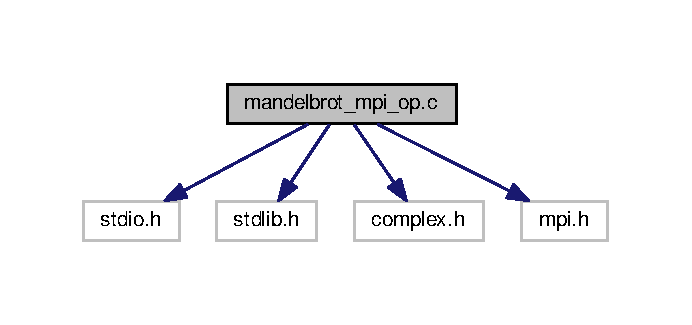
\includegraphics[width=332pt]{mandelbrot__mpi__op_8c__incl}
\end{center}
\end{figure}
\subsection*{Macros}
\begin{DoxyCompactItemize}
\item 
\#define {\bfseries M\+A\+X\+\_\+\+I\+T\+ER}~300\hypertarget{mandelbrot__mpi__op_8c_acd517c6f195c75b9dd0f3aad65326f3b}{}\label{mandelbrot__mpi__op_8c_acd517c6f195c75b9dd0f3aad65326f3b}

\item 
\#define {\bfseries E\+S\+C\+A\+P\+E\+\_\+\+R\+A\+D\+I\+U\+S\+\_\+\+S\+Q\+U\+A\+R\+ED}~4\hypertarget{mandelbrot__mpi__op_8c_a7c7393421319c3452cfbe9a49a5fbfa7}{}\label{mandelbrot__mpi__op_8c_a7c7393421319c3452cfbe9a49a5fbfa7}

\end{DoxyCompactItemize}
\subsection*{Functions}
\begin{DoxyCompactItemize}
\item 
int \hyperlink{mandelbrot__mpi__op_8c_a790aaf32862890d4cd0539c2a77149d6}{mandelbrot} (complex z0)
\begin{DoxyCompactList}\small\item\em Perform the calculations for the set until divergence or M\+A\+X\+\_\+\+I\+T\+ER. \end{DoxyCompactList}\item 
void \hyperlink{mandelbrot__mpi__op_8c_a2eb771fa3527f72e821a14e413498d1d}{print\+\_\+instructions} ()
\begin{DoxyCompactList}\small\item\em Function responsible for printing usage instructions. \end{DoxyCompactList}\item 
int {\bfseries main} (int argc, char $\ast$$\ast$argv)\hypertarget{mandelbrot__mpi__op_8c_a3c04138a5bfe5d72780bb7e82a18e627}{}\label{mandelbrot__mpi__op_8c_a3c04138a5bfe5d72780bb7e82a18e627}

\end{DoxyCompactItemize}


\subsection{Detailed Description}
Open M\+PI C implementation to compute and plot mandelbrot set. 

Open M\+PI C implementation of a program to compute and plot some subset of a mandelbrot set adapted from the classes given by MJ Rutter (\href{https://www.tcm.phy.cam.ac.uk/~mjr/courses/MPI/MPI.pdf}{\tt https\+://www.\+tcm.\+phy.\+cam.\+ac.\+uk/$\sim$mjr/courses/\+M\+P\+I/\+M\+P\+I.\+pdf}) in which every processes is responsible for writing your work with optimizations in the load balance

Usage\+: mpirun -\/np NP ./mandelbrot\+\_\+mpi\+\_\+op c\+\_\+x\+\_\+min c\+\_\+x\+\_\+max c\+\_\+y\+\_\+min c\+\_\+y\+\_\+max image\+\_\+size
\begin{DoxyItemize}
\item NP\+: Number of Open M\+PI processes
\item c\+\_\+x\+\_\+min\+: Lowest x boundary for the figure to be computed
\item c\+\_\+x\+\_\+max\+: Highest x boundary for the figure to be computed
\item c\+\_\+y\+\_\+mix\+: Lowest y boundary for the figure to be computed
\item c\+\_\+y\+\_\+max\+: Highest y boundary for the figure to be computed
\item image\+\_\+size\+: The resolution of the resulting image Usage examples\+: Full Picture\+: mpirun -\/np 4 ./mandelbrot\+\_\+mpi\+\_\+op -\/2.\+5 1.\+5 -\/2.\+0 2.\+0 11500 Seahorse Valley\+: mpirun -\/np 4 ./mandelbrot\+\_\+mpi\+\_\+op -\/0.\+8 -\/0.\+7 0.\+05 0.\+15 8192 Elephant Valley\+: mpirun -\/np 8 ./mandelbrot\+\_\+mpi\+\_\+op 0.\+175 0.\+375 -\/0.\+1 0.\+1 800 T Spir Val\+: mpirun -\/np 2 ./mandelbrot\+\_\+mpi\+\_\+op -\/0.\+188 -\/0.\+012 0.\+554 0.\+754 400
\end{DoxyItemize}

Notes\+: Although we made modifications, this code is heavily based on the class examples provided by MJ Rutter. Because of that, in any event of license and copyright conflict, the license/copyright provided by Mr. Rutter T\+A\+KE P\+R\+E\+C\+E\+D\+E\+N\+CE O\+V\+ER the G\+P\+Lv3 on which this code was released.

\begin{DoxyAuthor}{Author}
Decio Lauro Soares (\href{mailto:deciolauro@gmail.com}{\tt deciolauro@gmail.\+com}) 
\end{DoxyAuthor}
\begin{DoxyDate}{Date}
05 Jul 2017 
\end{DoxyDate}
\begin{DoxyRefDesc}{Bug}
\item[\hyperlink{bug__bug000005}{Bug}]No known bugs \end{DoxyRefDesc}
\begin{DoxyWarning}{Warning}
Based on class given by MJ Rutter(\+May contain Copyright issues) 
\end{DoxyWarning}
\begin{DoxyCopyright}{Copyright}
G\+NU Public License v3 
\end{DoxyCopyright}


\subsection{Function Documentation}
\index{mandelbrot\+\_\+mpi\+\_\+op.\+c@{mandelbrot\+\_\+mpi\+\_\+op.\+c}!mandelbrot@{mandelbrot}}
\index{mandelbrot@{mandelbrot}!mandelbrot\+\_\+mpi\+\_\+op.\+c@{mandelbrot\+\_\+mpi\+\_\+op.\+c}}
\subsubsection[{\texorpdfstring{mandelbrot(complex z0)}{mandelbrot(complex z0)}}]{\setlength{\rightskip}{0pt plus 5cm}int mandelbrot (
\begin{DoxyParamCaption}
\item[{complex}]{z0}
\end{DoxyParamCaption}
)}\hypertarget{mandelbrot__mpi__op_8c_a790aaf32862890d4cd0539c2a77149d6}{}\label{mandelbrot__mpi__op_8c_a790aaf32862890d4cd0539c2a77149d6}


Perform the calculations for the set until divergence or M\+A\+X\+\_\+\+I\+T\+ER. 

For the complex number z0, it performs the Mandelbrot calculation until it reaches divergence or it reaches the maximum number of iterations, whichever happens first, returning the number of iterations until divergence or M\+A\+X\+\_\+\+I\+T\+ER


\begin{DoxyParams}{Parameters}
{\em z0} & complex number to perform the Mandelbrot calculations \\
\hline
\end{DoxyParams}
\begin{DoxyReturn}{Returns}
i integer with the number of iterations until divergerce or M\+A\+X\+\_\+\+I\+T\+ER 
\end{DoxyReturn}
\index{mandelbrot\+\_\+mpi\+\_\+op.\+c@{mandelbrot\+\_\+mpi\+\_\+op.\+c}!print\+\_\+instructions@{print\+\_\+instructions}}
\index{print\+\_\+instructions@{print\+\_\+instructions}!mandelbrot\+\_\+mpi\+\_\+op.\+c@{mandelbrot\+\_\+mpi\+\_\+op.\+c}}
\subsubsection[{\texorpdfstring{print\+\_\+instructions()}{print_instructions()}}]{\setlength{\rightskip}{0pt plus 5cm}void print\+\_\+instructions (
\begin{DoxyParamCaption}
{}
\end{DoxyParamCaption}
)}\hypertarget{mandelbrot__mpi__op_8c_a2eb771fa3527f72e821a14e413498d1d}{}\label{mandelbrot__mpi__op_8c_a2eb771fa3527f72e821a14e413498d1d}


Function responsible for printing usage instructions. 

This function is responsible for printing the usage instructions 
\hypertarget{mandelbrot__seq_8c}{}\section{mandelbrot\+\_\+seq.\+c File Reference}
\label{mandelbrot__seq_8c}\index{mandelbrot\+\_\+seq.\+c@{mandelbrot\+\_\+seq.\+c}}


Sequential program to compute and plot mandelbrot set.  


{\ttfamily \#include $<$stdio.\+h$>$}\\*
{\ttfamily \#include $<$stdlib.\+h$>$}\\*
{\ttfamily \#include $<$complex.\+h$>$}\\*
Include dependency graph for mandelbrot\+\_\+seq.\+c\+:
\nopagebreak
\begin{figure}[H]
\begin{center}
\leavevmode
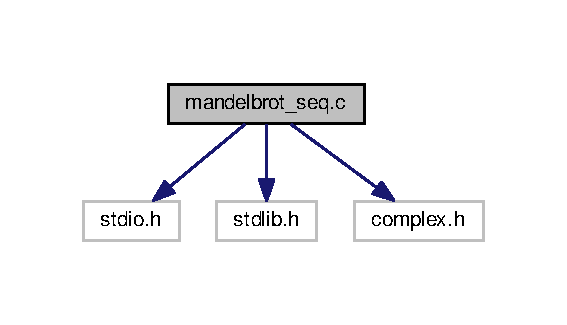
\includegraphics[width=272pt]{mandelbrot__seq_8c__incl}
\end{center}
\end{figure}
\subsection*{Macros}
\begin{DoxyCompactItemize}
\item 
\#define {\bfseries M\+A\+X\+\_\+\+I\+T\+ER}~300\hypertarget{mandelbrot__seq_8c_acd517c6f195c75b9dd0f3aad65326f3b}{}\label{mandelbrot__seq_8c_acd517c6f195c75b9dd0f3aad65326f3b}

\item 
\#define {\bfseries E\+S\+C\+A\+P\+E\+\_\+\+R\+A\+D\+I\+U\+S\+\_\+\+S\+Q\+U\+A\+R\+ED}~4\hypertarget{mandelbrot__seq_8c_a7c7393421319c3452cfbe9a49a5fbfa7}{}\label{mandelbrot__seq_8c_a7c7393421319c3452cfbe9a49a5fbfa7}

\end{DoxyCompactItemize}
\subsection*{Functions}
\begin{DoxyCompactItemize}
\item 
int \hyperlink{mandelbrot__seq_8c_a790aaf32862890d4cd0539c2a77149d6}{mandelbrot} (complex z0)
\begin{DoxyCompactList}\small\item\em Perform the calculations for the set until divergence or M\+A\+X\+\_\+\+I\+T\+ER. \end{DoxyCompactList}\item 
void \hyperlink{mandelbrot__seq_8c_a2eb771fa3527f72e821a14e413498d1d}{print\+\_\+instructions} ()
\begin{DoxyCompactList}\small\item\em Function responsible for printing usage instructions. \end{DoxyCompactList}\item 
int {\bfseries main} (int argc, char $\ast$$\ast$argv)\hypertarget{mandelbrot__seq_8c_a3c04138a5bfe5d72780bb7e82a18e627}{}\label{mandelbrot__seq_8c_a3c04138a5bfe5d72780bb7e82a18e627}

\end{DoxyCompactItemize}


\subsection{Detailed Description}
Sequential program to compute and plot mandelbrot set. 

C implementation of a sequential program to compute and plot some subset of a mandelbrot set adapted from the classes given by MJ Rutter (\href{https://www.tcm.phy.cam.ac.uk/~mjr/courses/MPI/MPI.pdf}{\tt https\+://www.\+tcm.\+phy.\+cam.\+ac.\+uk/$\sim$mjr/courses/\+M\+P\+I/\+M\+P\+I.\+pdf})

Usage\+: ./mandelbrot\+\_\+seq c\+\_\+x\+\_\+min c\+\_\+x\+\_\+max c\+\_\+y\+\_\+min c\+\_\+y\+\_\+max image\+\_\+size
\begin{DoxyItemize}
\item c\+\_\+x\+\_\+min\+: Lowest x boundary for the figure to be computed
\item c\+\_\+x\+\_\+max\+: Highest x boundary for the figure to be computed
\item c\+\_\+y\+\_\+mix\+: Lowest y boundary for the figure to be computed
\item c\+\_\+y\+\_\+max\+: Highest y boundary for the figure to be computed
\item image\+\_\+size\+: The resolution of the resulting image Usage examples\+: Full Picture\+: ./mandelbrot\+\_\+seq -\/2.\+5 1.\+5 -\/2.\+0 2.\+0 11500 Seahorse Valley\+: ./mandelbrot\+\_\+seq -\/0.\+8 -\/0.\+7 0.\+05 0.\+15 11500 Elephant Valley\+: ./mandelbrot\+\_\+seq 0.\+175 0.\+375 -\/0.\+1 0.\+1 11500 Triple Spiral Valley\+: ./mandelbrot\+\_\+seq -\/0.\+188 -\/0.\+012 0.\+554 0.\+754 11500
\end{DoxyItemize}

Notes\+: Although we made modifications, this code is heavily based on the class examples provided by MJ Rutter. Because of that, in any event of license and copyright conflict, the license/copyright provided by Mr. Rutter T\+A\+KE P\+R\+E\+C\+E\+D\+E\+N\+CE O\+V\+ER the G\+P\+Lv3 on which this code was released.

\begin{DoxyAuthor}{Author}
Decio Lauro Soares (\href{mailto:deciolauro@gmail.com}{\tt deciolauro@gmail.\+com}) 
\end{DoxyAuthor}
\begin{DoxyDate}{Date}
05 Jul 2017 
\end{DoxyDate}
\begin{DoxyRefDesc}{Bug}
\item[\hyperlink{bug__bug000006}{Bug}]No known bugs \end{DoxyRefDesc}
\begin{DoxyWarning}{Warning}
Based on class given by MJ Rutter(\+May contain Copyright issues) 
\end{DoxyWarning}
\begin{DoxyCopyright}{Copyright}
G\+NU Public License v3 
\end{DoxyCopyright}


\subsection{Function Documentation}
\index{mandelbrot\+\_\+seq.\+c@{mandelbrot\+\_\+seq.\+c}!mandelbrot@{mandelbrot}}
\index{mandelbrot@{mandelbrot}!mandelbrot\+\_\+seq.\+c@{mandelbrot\+\_\+seq.\+c}}
\subsubsection[{\texorpdfstring{mandelbrot(complex z0)}{mandelbrot(complex z0)}}]{\setlength{\rightskip}{0pt plus 5cm}int mandelbrot (
\begin{DoxyParamCaption}
\item[{complex}]{z0}
\end{DoxyParamCaption}
)}\hypertarget{mandelbrot__seq_8c_a790aaf32862890d4cd0539c2a77149d6}{}\label{mandelbrot__seq_8c_a790aaf32862890d4cd0539c2a77149d6}


Perform the calculations for the set until divergence or M\+A\+X\+\_\+\+I\+T\+ER. 

For the complex number z0, it performs the Mandelbrot calculation until it reaches divergence or it reaches the maximum number of iterations, whichever happens first, returning the number of iterations until divergence or M\+A\+X\+\_\+\+I\+T\+ER


\begin{DoxyParams}{Parameters}
{\em z0} & complex number to perform the Mandelbrot calculations \\
\hline
\end{DoxyParams}
\begin{DoxyReturn}{Returns}
i integer with the number of iterations until divergerce or M\+A\+X\+\_\+\+I\+T\+ER 
\end{DoxyReturn}
\index{mandelbrot\+\_\+seq.\+c@{mandelbrot\+\_\+seq.\+c}!print\+\_\+instructions@{print\+\_\+instructions}}
\index{print\+\_\+instructions@{print\+\_\+instructions}!mandelbrot\+\_\+seq.\+c@{mandelbrot\+\_\+seq.\+c}}
\subsubsection[{\texorpdfstring{print\+\_\+instructions()}{print_instructions()}}]{\setlength{\rightskip}{0pt plus 5cm}void print\+\_\+instructions (
\begin{DoxyParamCaption}
{}
\end{DoxyParamCaption}
)}\hypertarget{mandelbrot__seq_8c_a2eb771fa3527f72e821a14e413498d1d}{}\label{mandelbrot__seq_8c_a2eb771fa3527f72e821a14e413498d1d}


Function responsible for printing usage instructions. 

This function is responsible for printing the usage instructions 
%--- End generated contents ---

% Index
\backmatter
\newpage
\phantomsection
\clearemptydoublepage
\addcontentsline{toc}{chapter}{Index}
\printindex

\end{document}
